% Figure from MATH 452 notes, section 15. Compile with the notes preamble.
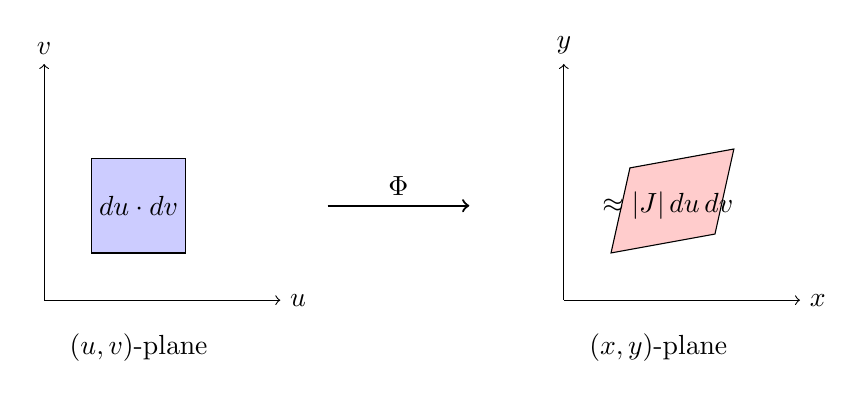
\begin{tikzpicture}[scale=1.2]
% Left: (u,v) plane
\draw[->] (0,0) -- (2.5,0) node[right] {$u$};
\draw[->] (0,0) -- (0,2.5) node[above] {$v$};
\draw[fill=blue!20] (0.5,0.5) rectangle (1.5,1.5);
\node at (1,1) {$du \cdot dv$};
\node at (1,-0.5) {$(u,v)$-plane};

% Arrow
\draw[->, thick] (3,1) -- (4.5,1) node[midway, above] {$\Phi$};

% Right: (x,y) plane
\begin{scope}[xshift=5.5cm]
\draw[->] (0,0) -- (2.5,0) node[right] {$x$};
\draw[->] (0,0) -- (0,2.5) node[above] {$y$};
\draw[fill=red!20] (0.5,0.5) -- (1.6,0.7) -- (1.8,1.6) -- (0.7,1.4) -- cycle;
\node at (1.1,1) {$\approx |J| \, du \, dv$};
\node at (1,-0.5) {$(x,y)$-plane};
\end{scope}
\end{tikzpicture}
